\documentclass[11pt, aspectratio=169]{beamer}

\usepackage{amsmath, amsfonts, microtype, nicefrac, amssymb, amsthm, centernot}

\usepackage{pgfpages}

\usepackage{helvet}
\usepackage[default]{lato}
\usepackage{array}

\usefonttheme[onlymath]{serif}

\usepackage[utf8]{inputenc}
\usepackage[T1]{fontenc}
\usepackage{textcomp}
\usepackage{bm}

\usepackage{mathpazo}
\usepackage{hyperref}
\usepackage{multimedia}
\usepackage{graphicx}
\usepackage{multirow}
\usepackage{graphicx}
\usepackage{dcolumn}
\usepackage{bbm}
\newcolumntype{d}[0]{D{.}{.}{5}}

\usepackage{graphicx}
\usepackage[space]{grffile}
\usepackage{booktabs}

\usepackage{setspace}

\usepackage{transparent}


%%% FIGURES %%%
\usepackage{caption, subcaption}
\usepackage{booktabs, siunitx}
\usepackage{pgfplots} 
%\usepackage[outdir=./figures]{epstopdf}
\usepackage{float}
\usepackage{graphicx}
\usepackage[absolute, overlay]{textpos}
\usepackage{epstopdf}


%%% TIKZ %%%
\usepackage{tikz}
\usepackage{verbatim}
\usetikzlibrary{arrows.meta}
\usetikzlibrary{positioning}
\usetikzlibrary{bending}
\usetikzlibrary{snakes}
\usetikzlibrary{calc}
\usetikzlibrary{arrows}
\usetikzlibrary{decorations.markings}
\usetikzlibrary{shapes.misc}
\usetikzlibrary{matrix, shapes, arrows, fit, tikzmark}


%%% ALGORITHM %%%
\usepackage{algorithm}
\usepackage[noend]{algpseudocode}
\usepackage{multimedia}


%%% APPENDIX SLIDE NUMBERING %%%
\usepackage{appendixnumberbeamer}


%%% BEAMER BUTTON %%%
%\setbeamertemplate{button}{\tikz
	%\node[
	%	inner xsep = 2pt, 
	%	draw = structure!0, 
	%	fill = myblue, 
	%	rounded corners = 4pt]{\color{white} \tiny\insertbuttontext};
	%}


%%% COLORS %%%
\definecolor{blue}{RGB}{0,38,118}
\definecolor{red}{RGB}{213,94,0}
\definecolor{yellow}{RGB}{240,228,66}
\definecolor{green}{RGB}{0,158,115}

\definecolor{myred}{RGB}{163,32,45}
\definecolor{navyblue}{rgb}{0.05,0.2,0.70}
\definecolor{myblue}{RGB}{0,51,150}
\definecolor{myorange}{RGB}{255,140,0}
\definecolor{myref}{RGB}{160,160,160}
\definecolor{shock}{RGB}{0, 125, 34}%{50, 168, 82}

\definecolor{background}{RGB}{255,253,218}

% Define a new transparent color
\definecolor{trans}{rgb}{1,1,1}
\colorlet{trans}{black!20} % 0 percent opacity

\hypersetup{
  colorlinks=false,
  linkbordercolor = {white},
  linkcolor = {blue}
}

\setbeamercolor{frametitle}{fg=blue}
\setbeamercolor{title}{fg=black}
\setbeamertemplate{footline}[frame number]
\setbeamertemplate{navigation symbols}{} 
\setbeamertemplate{itemize items}{-}
\setbeamercolor{itemize item}{fg=blue}
\setbeamercolor{itemize subitem}{fg=blue}
\setbeamercolor{enumerate item}{fg=blue}
\setbeamercolor{enumerate subitem}{fg=blue}
\setbeamercolor{button}{bg=background, fg=blue,}

%\setbeamercolor{background canvas}{bg=background}


%%% FRAME TITLE %%%
\setbeamerfont{title}{series=\bfseries, parent=structure}
\setbeamerfont{frametitle}{series=\bfseries, parent=structure}


%%% TRANSITION FRAME %%%
\newenvironment{transitionframe}{
	\setbeamercolor{background canvas}{bg=blue}
	\begin{frame}
		\thispagestyle{empty}
		\addtocounter{framenumber}{-1}
		\vspace{42mm}
		\hspace{4mm} }{
		\begin{tikzpicture}
			\tikz \fill [white] (1,6) rectangle (20,10);
		\end{tikzpicture}
	\end{frame}
}


%%% OUTLINE %%%
\AtBeginSection[]
{
	\begin{frame}
       \frametitle{Roadmap of Talk}
       \tableofcontents[currentsection]
   \end{frame}
}
\setbeamercolor{section in toc}{fg=blue}
\setbeamercolor{subsection in toc}{fg=red}
\setbeamersize{text margin left=1em,text margin right=1em} 


%%% ENVIRONMENTS
\newenvironment{witemize}{\itemize\addtolength{\itemsep}{10pt}}{\enditemize}

\makeatother
\setbeamertemplate{itemize items}{\large\raisebox{0mm}{\textbullet}}
\setbeamertemplate{itemize subitem}{\footnotesize\raisebox{0.15ex}{--}}
\setbeamertemplate{itemize subsubitem}{\Tiny\raisebox{0.7ex}{$\blacktriangleright$}}

\setbeamertemplate{enumerate item}[default]
\setbeamertemplate{enumerate subitem}{\textbullet}
\makeatletter

% ITEMIZE SPACING:
% \usepackage{xpatch}
% \xpatchcmd{\itemize}
% {\def\makelabel}
% {\setlength{\itemsep}{0mm}\def\makelabel}
% {}
% {}


%%% PRETTY ENUMERATE %%%
% \usepackage{stackengine,xcolor}
% \newcommand\circnum[2]{\stackinset{c}{}{c}{.1ex}{\small\textcolor{white}{#2}}%
	% 	{\abovebaseline[-.7ex]{\Huge\textcolor{#1}{$\bullet$}}}}
% \newenvironment{myenum}
% {\let\svitem\item
	% 	\renewcommand\item[1][black]{%
		% 		\refstepcounter{enumi}\svitem[\circnum{##1}{\theenumi}]}%
	% 	\begin{enumerate}}{\end{enumerate}}
\usepackage{stackengine,xcolor,graphicx}
\newcommand\circnum[2]{\smash{\stackinset{c}{}{c}{.2ex}{\small\textcolor{white}{#2}}%
		{\abovebaseline[-1.1ex]{\Huge\textcolor{#1}{\scalebox{1.5}{$\bullet$}}}}}}
\newenvironment{myenum}
{\let\svitem\item
	\renewcommand\item[1][black]{%
		\refstepcounter{enumi}\svitem[\circnum{##1}{\theenumi}]}%
	\begin{enumerate}}{\end{enumerate}}

\newcommand{\notimplies}{\;\not\!\!\!\implies}



%%%%%%%%%%%%%%%%%%%%%%%%%%  TITLE   %%%%%%%%%%%%%%%%%%%%%%%%%%%%%%%%
\title[]{\\[8pt]
	{\large \color{blue} Dynamic Programming and Applications \\[5pt] \normalfont{Stochastic Dynamic Programming in Continuous Time} \\[10pt] \normalfont{Lectures 5 -- 6}}}
\author[Schaab]{Andreas Schaab}
\institute{}
\subject{}
\date{}



%%%%%%%%%%%%%%%%%%%%%%%%  BEGIN DOC   %%%%%%%%%%%%%%%%%%%%%%%%%%%%%%%
\begin{document}

%%% TIKZ %%% 
\tikzstyle{every picture}+=[remember picture]
%\everymath{\displaystyle}

\tikzset{   
	every picture/.style={remember picture,baseline},
	every node/.style={anchor=base,align=center,outer sep=1.5pt},
	every path/.style={thick},
}
\newcommand\marktopleft[1]{%
	\tikz[overlay,remember picture] 
	\node (marker-#1-a) at (-.3em,.3em) {};%
}
\newcommand\markbottomright[2]{%
	\tikz[overlay,remember picture] 
	\node (marker-#1-b) at (0em,0em) {};%
}
\tikzstyle{every picture}+=[remember picture] 
\tikzstyle{mybox} =[draw=black, very thick, rectangle, inner sep=10pt, inner ysep=20pt]
\tikzstyle{fancytitle} =[draw=black,fill=red, text=white]


\addtocounter{framenumber}{-1}
\thispagestyle{empty}
\maketitle 
\newpage




%%%%%%%%%%%%%%%%%%%%%%%%%%  SLIDE   %%%%%%%%%%%%%%%%%%%%%%%%%%%%%%%%
\begin{frame}{Outline}
\thispagestyle{empty}
\addtocounter{framenumber}{-1}

Part 1: Stochastic processes, Brownian motion, and stochastic differential equations
\begin{enumerate}
	\item Stochastic processes in continuous time
	\item Continuous time Markov chains
	\item Brownian motion
	\item Diffusion processes 
	\item Ito's Lemma
	\item Poisson processes
	\item The generator of a stochastic process
\end{enumerate}

\end{frame}


%%%%%%%%%%%%%%%%%%%%%%%%%%  SLIDE   %%%%%%%%%%%%%%%%%%%%%%%%%%%%%%%%
\begin{frame}{Outline}
\thispagestyle{empty}
\addtocounter{framenumber}{-1}

Part 2: Optimization with stochastic dynamics
\begin{enumerate}
	\item Stochastic neoclassical growth model
	\item Stochastic neoclassical growth with diffusion process
	\item Stochastic neoclassical growth with Poisson process
\end{enumerate}

\end{frame}

%%%%%%%%%%%%%%%%%%%%%%%%%%  SLIDE   %%%%%%%%%%%%%%%%%%%%%%%%%%%%%%%%
\begin{frame}{Outline}
\thispagestyle{empty}
\addtocounter{framenumber}{-1}

Part 3: Applications
\begin{enumerate}
	\item Consumption-savings with stochastic income fluctuations
	\item Firm profit maximization
	\item Capital investment with adjustment cost
	\item Investing in stocks
	\item Real business cycles
	\item AK technology 
\end{enumerate}

\end{frame}


%%%%%%%%%%%%%%%%%%%%%%%%%%  SLIDE   %%%%%%%%%%%%%%%%%%%%%%%%%%%%%%%%
\begin{transitionframe}
	{\color{white} \Huge \textbf{Part 1: Stochastic Processes} \vspace{2mm}}
\end{transitionframe}


%%%%%%%%%%%%%%%%%%%%%%%%%%  SLIDE   %%%%%%%%%%%%%%%%%%%%%%%%%%%%%%%%
\begin{frame}{1. Stochastic processes in continuous time} 

\textbf{Definition.} A \textbf{stochastic process} is a time-indexed sequence of random variables.

\vspace{5mm}
\begin{witemize}
\item A random variable maps an ``event'' into a scalar, a stochastic process maps an event into a path 
	
\item Formally, an event is $\omega \in \Omega$ and a random variable $X: \Omega \to \mathbb R$ (learn some basic measure theory!)

\item A stochastic process is a sequence $\{ X_t \}_{t \geq 0}$ such that each $X_t$ is a random variable. In discrete time $t \in \{0, 1, \ldots\}$ and in continuous time $t \in [0, \infty)$

\item We can also think of a stochastic process as a random variable, but one that maps into a different space---a function space!
\end{witemize}
\end{frame}


%%%%%%%%%%%%%%%%%%%%%%%%%%  SLIDE   %%%%%%%%%%%%%%%%%%%%%%%%%%%%%%%%
\begin{frame}{}

\textbf{Definition.} Let $X = \{X_t\}_{t \geq 0}$ be a sequence of random variables taking values in a finite or countable state space $\mathcal X$. Then $X$ is a \textit{continuous-time Markov chain} if it satisfies the \textit{Markov property}: For any sequence $0 \leq t_1 < t_2 < \ldots < t_n$ of times 
\begin{equation*}
	\mathbb P(X_{t_n} = x \mid X_{t_1}, \ldots, X_{t_{n-1}} ) = \mathbb P(X_{t_n} = x \mid X_{t_{n-1}} )
\end{equation*}


\vspace{5mm}
\textbf{Definition.} Process $X$ is \textbf{time-homogeneous} or \textbf{stationary} if the conditional probability does not depend on the current time, i.e., for $x, y \in \mathcal X$:
\begin{equation*}
	\mathbb P(X_{t+s} = x \mid X_s = y) = \mathbb P(X_t = x \mid X_0 = y)
\end{equation*}

\begin{witemize}
\item Alternatively: If all possible joint distributions are independent of time $t$.
\end{witemize}
\end{frame}


%%%%%%%%%%%%%%%%%%%%%%%%%%  SLIDE   %%%%%%%%%%%%%%%%%%%%%%%%%%%%%%%%
\begin{frame}{}
\begin{witemize}
\item The \textit{transition density} of process $X$ is denoted $p(t, x \mid s, y)$ and is defined as 
\begin{equation*}
	\mathbb P(X_t \in A \mid Y_s = y) = \int_A p(t, x \mid s, y) dx 
\end{equation*}
for any (Borel) set $A \subset \mathcal X$. In words: $p(t, x \mid s, y)$ is the probability (density) that process $X_t$ ends up at $X_t = x$ at time $t$ if it started at $X_s = y$ at time $s$

\item \textit{Conditional expectation} can be written as: $\mathbb E[ f(X_t) \mid X_0 = y] = \int p(t, x \mid 0, y) f(x) dx$
\end{witemize}
\end{frame}


%%%%%%%%%%%%%%%%%%%%%%%%%%  SLIDE   %%%%%%%%%%%%%%%%%%%%%%%%%%%%%%%%
\begin{frame}{}

\textbf{Definition.} A process $X$ is a \textbf{martingale} if it satisfies
\begin{equation*}
	\mathbb E \Big[ X_{t + s} \mid \text{ information available at } t \Big] = X_t
\end{equation*}

\vspace{5mm}
\begin{witemize}
\item The most important martingale in macroeconomics: Suppose $\beta R_t = 1$ then 
\begin{equation*}
	\mathbb E_t \Big[ u'(C_{t + s}) \Big] = u'(C_t).
\end{equation*}

\item Efficient markets hypothesis in finance $\approx$ $\mathbb E_t (P_{t + s}) = P_t$

\item A random walk is a martingale (but not every martingale is a random walk)
\end{witemize}
\end{frame}



%%%%%%%%%%%%%%%%%%%%%%%%%%  SLIDE   %%%%%%%%%%%%%%%%%%%%%%%%%%%%%%%%
\begin{frame}{}

\textbf{Example}: 

\vspace{5mm}
\begin{witemize}
\item Consider the two-state employment process $z_t \in \{z^L, z^H\}$ with transition rates $\lambda^{LH}$ (from L to H) and $\lambda^{HL}$ (from H to L)

\item The associated transition matrix (\textit{generator}) is 
\begin{equation*}
	\mathcal A^z = \begin{pmatrix} - \lambda^{LH} & \lambda^{LH} \\ \lambda^{HL} & -\lambda^{HL} \end{pmatrix}
\end{equation*}

\item Interpretation: households transition \textit{out of} state $i$ at rate $\lambda^{ij}$

\item Notice: In discrete time, Markov transition matrix rows sum to $1$. Here, rows sum to $0$ (\textit{mass preservation})
\end{witemize}
\end{frame}


%%%%%%%%%%%%%%%%%%%%%%%%%  SLIDE   %%%%%%%%%%%%%%%%%%%%%%%%%%%%%%
\begin{frame}{2. Brownian motion}
\begin{witemize}
\item Brownian motion is the most  

\item Einstein (1905) uses Brownian motion to model motion of particles

\item We will introduce / discuss Brownian motion from 3 perspectives
\end{witemize}
\end{frame}


%%%%%%%%%%%%%%%%%%%%%%%%%  SLIDE   %%%%%%%%%%%%%%%%%%%%%%%%%%%%%%
\begin{frame}{Brownian motion: perspective \#1}
\begin{witemize}
\item Consider a process $X(t)$. Every $\Delta$ time step, the process either goes up or down by $h$
\begin{equation*}
	\Delta X \equiv X(t+\Delta) - X(t) = 
	\begin{cases}
		+ h & \text{ with probability } p \\
		- h & \text{ with probability } q = 1-p
	\end{cases}
\end{equation*}

\item Then we have:
\begin{align*}
	\mathbb E(\Delta X) &= ph - qh = (p-q)h \\
	\mathbb E((\Delta X)^2) &= ph^2 + qh^2 = h^2 \\
	Var(\Delta X) &= \mathbb E[ \Delta X - \mathbb E (\Delta X)]^2 = 4 pq h^2
\end{align*}

\end{witemize}
\end{frame}


%%%%%%%%%%%%%%%%%%%%%%%%%  SLIDE   %%%%%%%%%%%%%%%%%%%%%%%%%%%%%%
\begin{frame}{}
\begin{witemize}
\item Notice that $X(t) - X(0)$ is a binomial random variable with 
\begin{align*}
	\mathbb E[X(t) - X(0)] &= n(p - q) h = t(p-q) \frac{h}{\Delta} \\
	Var[X(t) - X(0)] &= n 4 pq h^2 = t 4 pq \frac{h^2}{\Delta}
\end{align*}
where $n = t / \Delta$ is the number of jumps in interval $[0, t]$

\item Next, let 
\begin{equation*}
	h = \sigma \sqrt{\Delta} 
	\quad \quad \text{ and } \quad\quad
	p = \frac{1}{2} \Big[ 1 + \frac{\mu}{\sigma} \sqrt{\Delta} \Big]
\end{equation*}

\item This implies
\begin{gather*}
(p-q) = \frac{\mu}{\sigma} \sqrt{\Delta} \\
	\mathbb E[X(t) - X(0)] = t \frac{\mu}{\sigma} \sqrt{\Delta} \sigma \frac{\sqrt{\Delta}}{\Delta} = \mu t \\
	Var[X(t) - X(0)] \longrightarrow_{\text{as} \Delta \to 0} \sigma^2 t
\end{gather*}

\end{witemize}
\end{frame}


%%%%%%%%%%%%%%%%%%%%%%%%%  SLIDE   %%%%%%%%%%%%%%%%%%%%%%%%%%%%%%
\begin{frame}{}
\textbf{Implications:}
\begin{witemize}
	\item Vertical movements proportional to $\sqrt{\Delta}$ not $\Delta$

	\item Convergence in distribution: $X(t) - X(0) \to^D \mathcal N(\mu t, \sigma t)$ since Binomial $\to^D$ Normal
		
	\item Distance traveled (length of curve) during $t \in [0, 1]$ is $= nh = \frac{1}{\Delta} \sigma \sqrt \Delta = \sigma \frac{1}{\sqrt \Delta} \to \infty$

	\item Time derivative $\mathbb E \frac{dX}{dt}$ doesn't exist: $\frac{\Delta X}{\Delta} = \frac{\pm \sigma \sqrt \Delta}{\Delta} = \frac{\pm \sigma}{\sqrt \Delta} \to \infty$

	\item $\frac{\mathbb E \Delta X}{\Delta} = \frac{\mu h^2 / \sigma^2}{\Delta} = \mu$ so we can write $\mathbb E(dX) = \mu dt$

	\item $\frac{Var(\Delta X)}{\Delta} \to \sigma^2$ so we can write $Var(dX) = \sigma^2 dt$
\end{witemize}
\end{frame}


%%%%%%%%%%%%%%%%%%%%%%%%%  SLIDE   %%%%%%%%%%%%%%%%%%%%%%%%%%%%%%
\begin{frame}{}
	\begin{figure}
		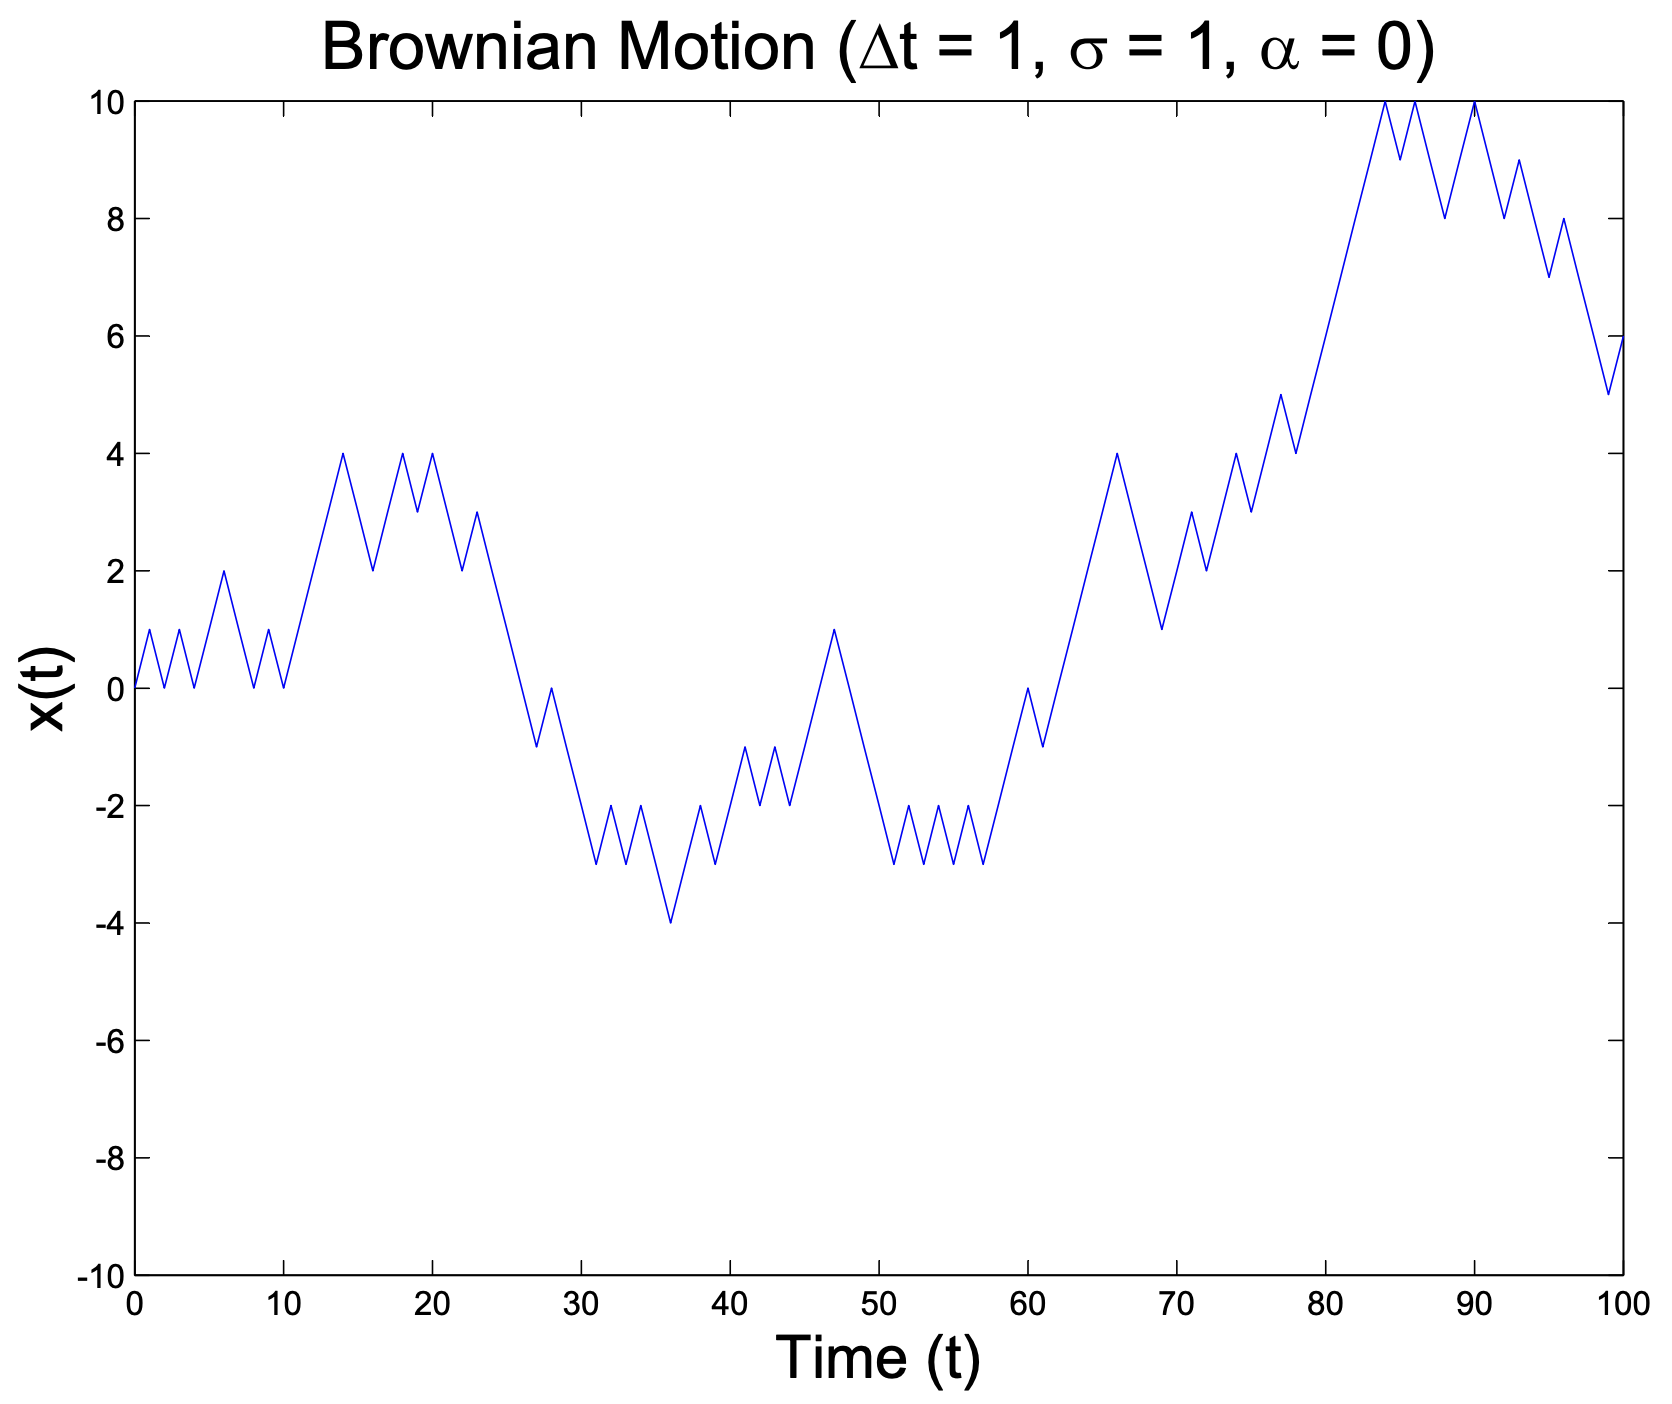
\includegraphics[scale=0.3]{./Brownian1}
	\end{figure}
\end{frame}


%%%%%%%%%%%%%%%%%%%%%%%%%  SLIDE   %%%%%%%%%%%%%%%%%%%%%%%%%%%%%%
\begin{frame}{}
	\begin{figure}
		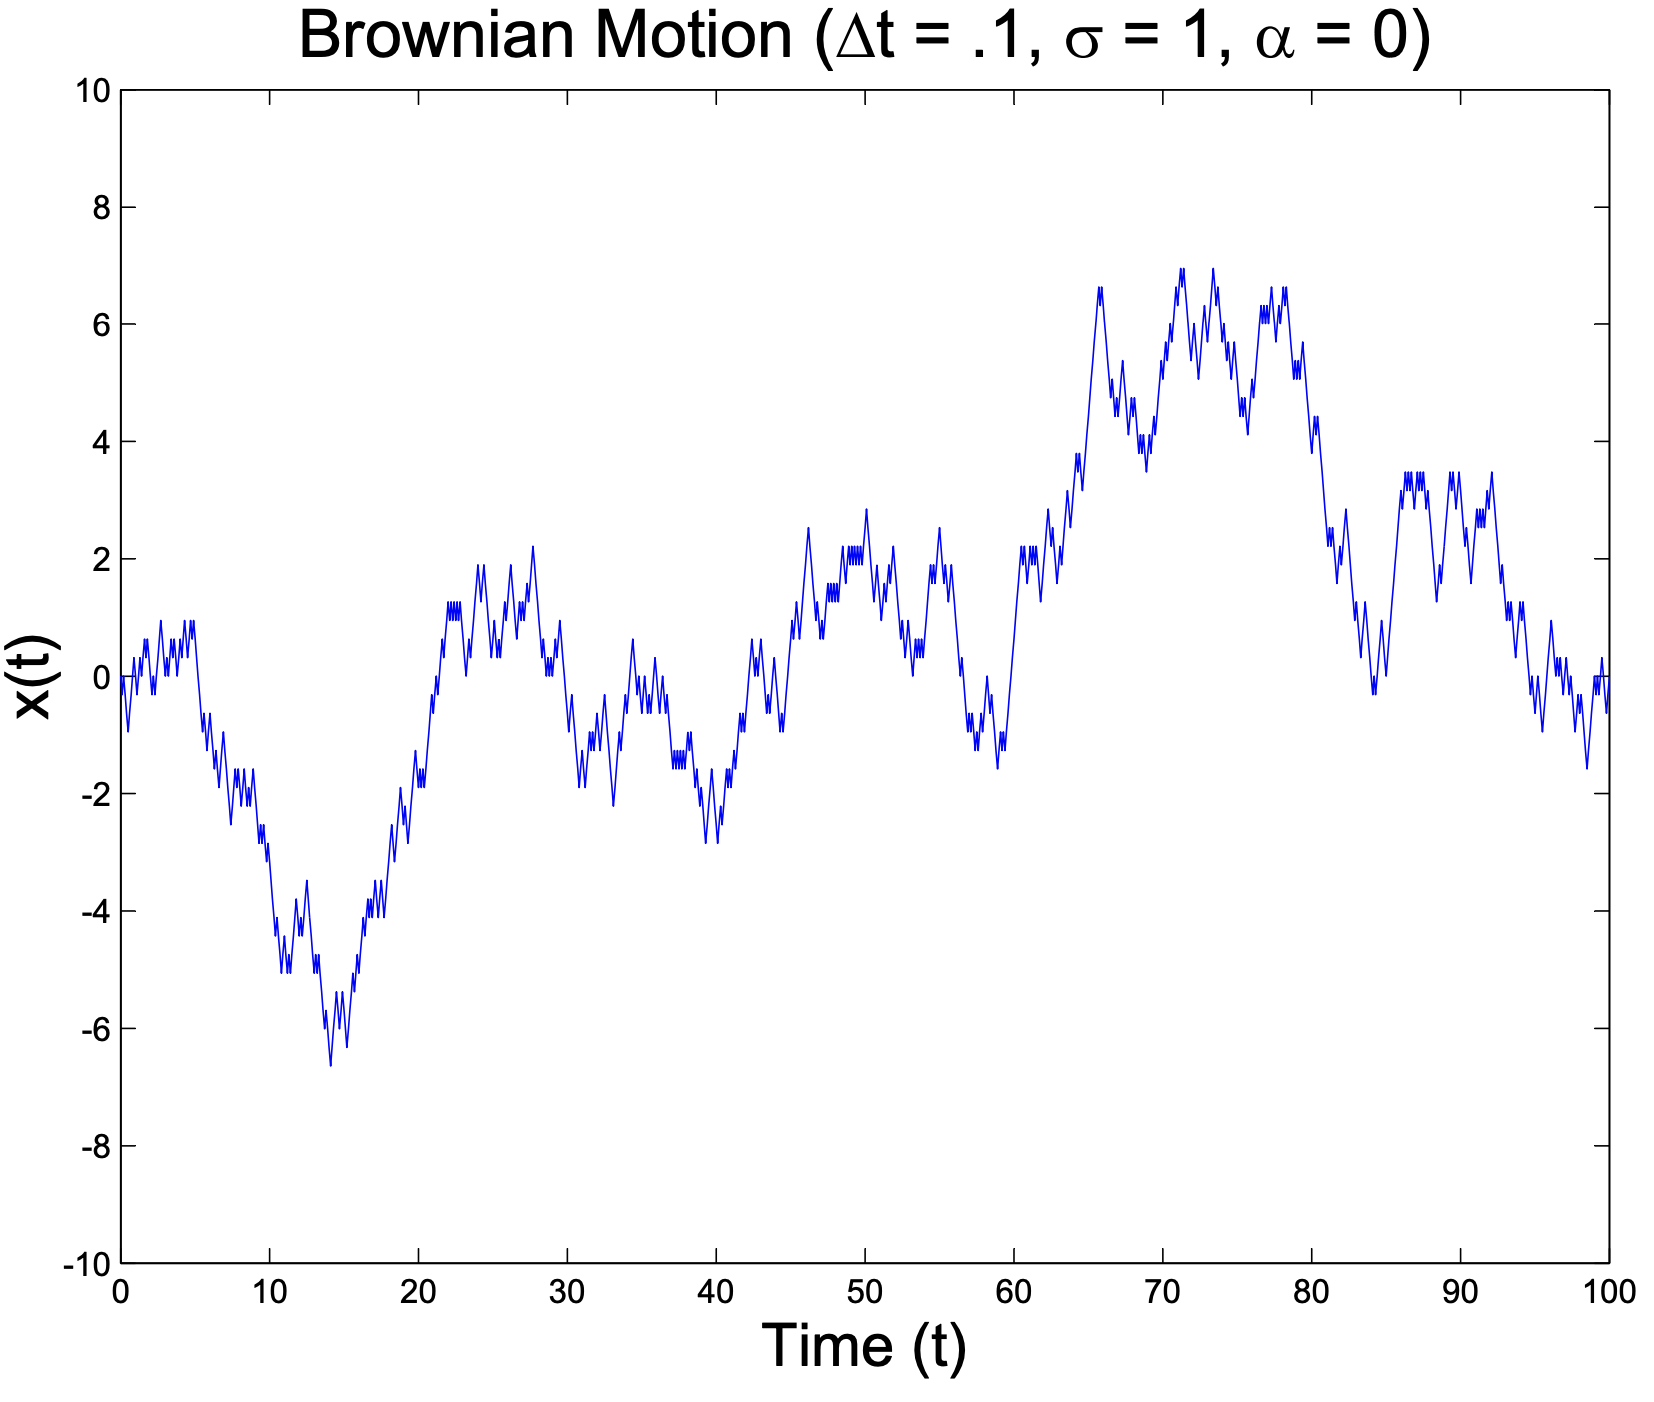
\includegraphics[scale=0.3]{./Brownian2}
	\end{figure}
\end{frame}


%%%%%%%%%%%%%%%%%%%%%%%%%  SLIDE   %%%%%%%%%%%%%%%%%%%%%%%%%%%%%%
\begin{frame}{}
	\begin{figure}
		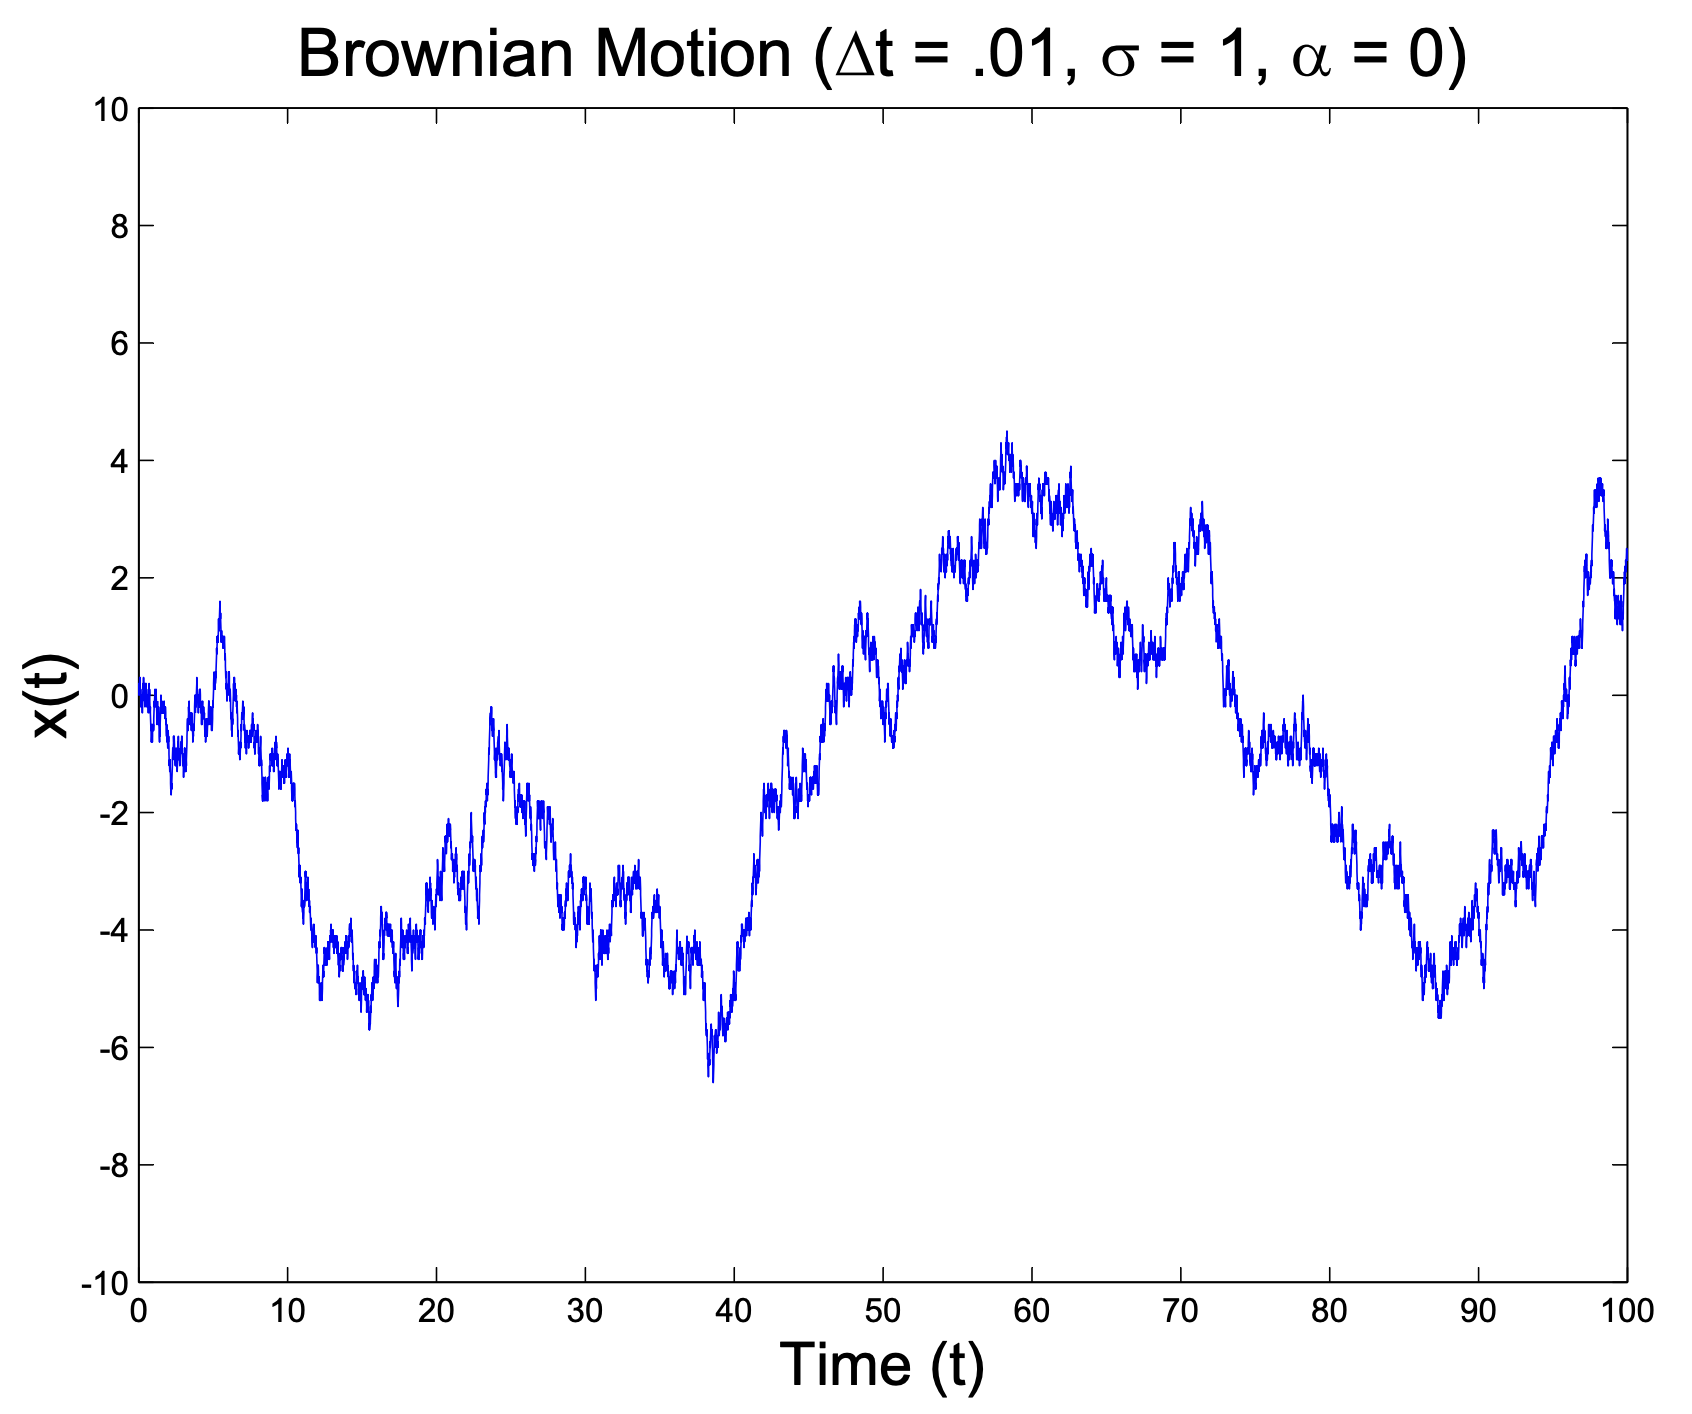
\includegraphics[scale=0.3]{./Brownian3}
	\end{figure}
\end{frame}


%%%%%%%%%%%%%%%%%%%%%%%%%  SLIDE   %%%%%%%%%%%%%%%%%%%%%%%%%%%%%%
\begin{frame}{}
	\begin{figure}
		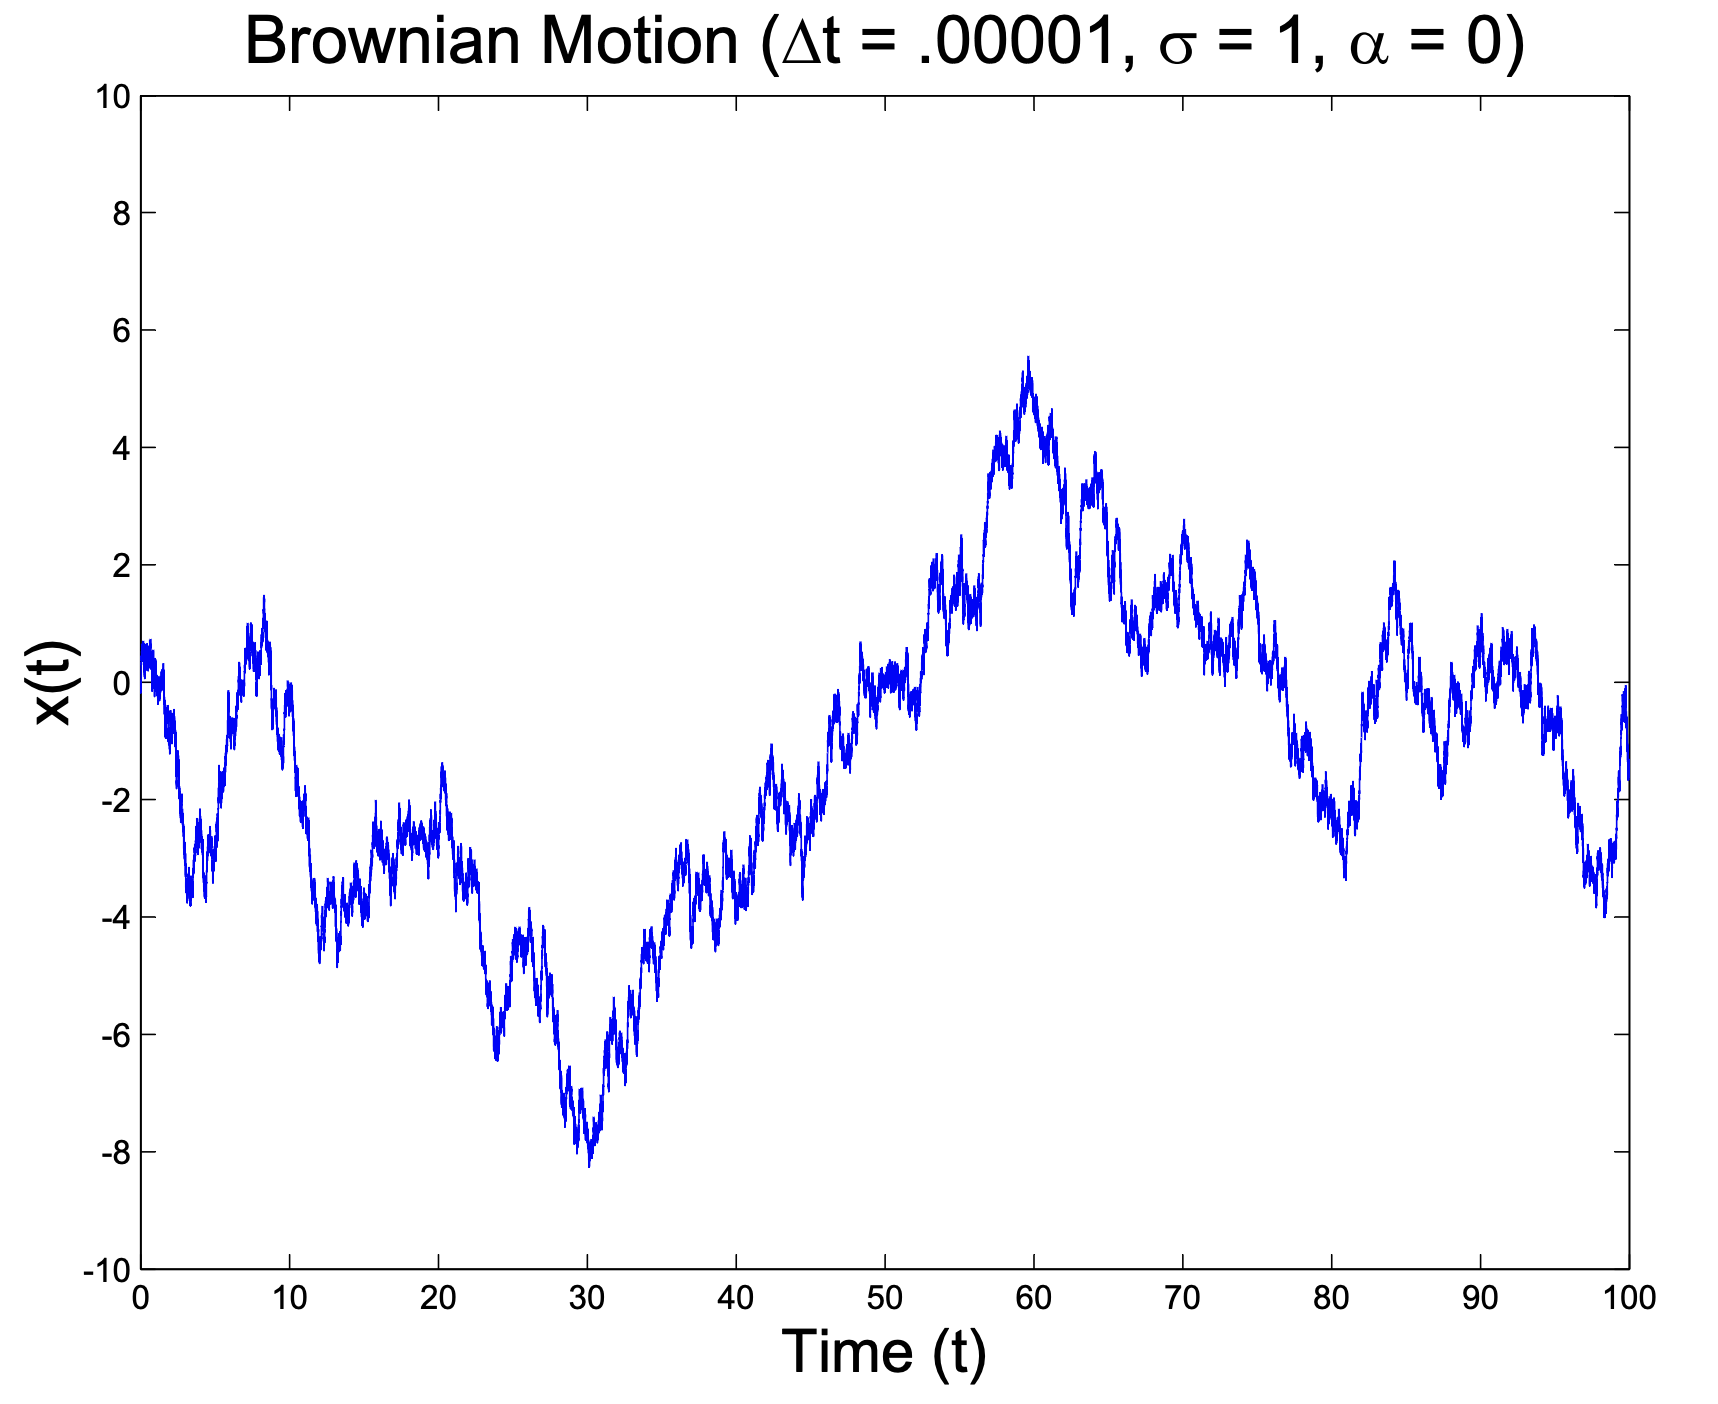
\includegraphics[scale=0.3]{./Brownian4}
	\end{figure}
\end{frame}


%%%%%%%%%%%%%%%%%%%%%%%%%  SLIDE   %%%%%%%%%%%%%%%%%%%%%%%%%%%%%%
\begin{frame}{Brownian motion: perspective \#2}
\begin{witemize}
\item Consider a random walk process in discrete time:
\begin{equation*}
	W_{t+1} = W_t + \epsilon_t, 
	\quad\quad \text{ where } 
	W_0 = 0 \text{ and } 
	\epsilon_t \sim \mathcal N(0, 1)
\end{equation*}

\item We can extend this to a generalized time step:
\begin{equation*}
	W_{t+\Delta} = W_t + \sqrt{\Delta} \epsilon_t, 
	\quad\quad \text{ where } 
	W_0 = 0 \text{ and } 
	\epsilon_t \sim \mathcal N(0, 1)
\end{equation*}

\item Why the square root? 
\begin{equation*}
	Var(W_{t + \Delta} - W_t) = Var(\sqrt{\Delta} \epsilon_t)
	= \Delta Var(\epsilon_t) = \Delta
	\quad \implies \quad
	Var(W_t) = t
\end{equation*}

\item You get Brownian motion by taking limit $\Delta \to 0$: Brownian motion = continuous time random walk
\end{witemize}
\end{frame}


%%%%%%%%%%%%%%%%%%%%%%%%%  SLIDE   %%%%%%%%%%%%%%%%%%%%%%%%%%%%%%
\begin{frame}{}
	\begin{figure}
		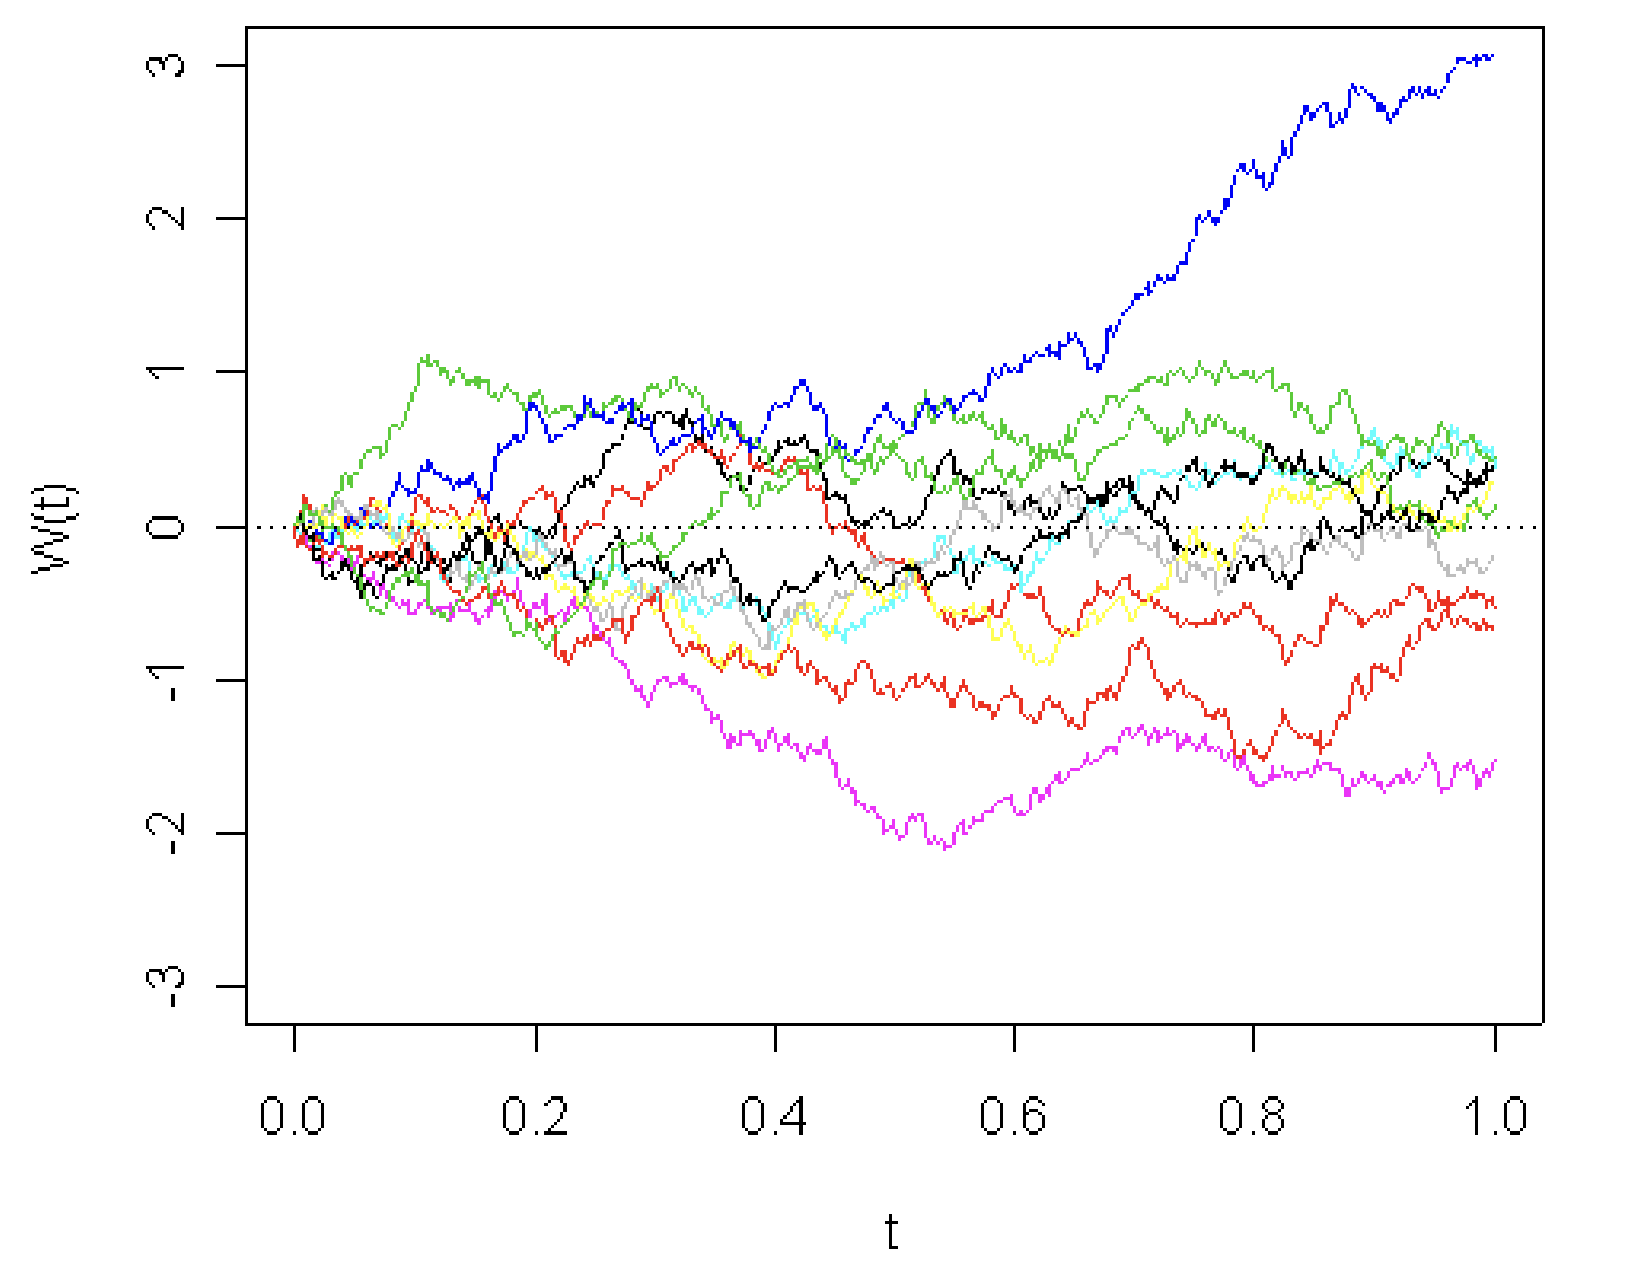
\includegraphics[scale=0.3]{./Brownian5}
	\end{figure}
\end{frame}


%%%%%%%%%%%%%%%%%%%%%%%%%  SLIDE   %%%%%%%%%%%%%%%%%%%%%%%%%%%%%%
\begin{frame}{Brownian motion: perspective \#3}

\vspace{4mm}
\textbf{Definition.} Brownian motion $\{B_t\}_{t\geq 0}$ is a stochastic process with properties:
\begin{witemize}
\item [(i)] $B_0 = 0$

\vspace{-3mm}
\item [(ii)] (\textit{Independent increments}) For non-overlapping $0 \leq t_1 < t_2 < t_3 < t_4$, we have $B_{t_2} - B_{t_1}$ independent from $B_{t_4} - B_{t_3}$

\vspace{-3mm}
\item [(iii)] (\textit{Normal, stationary increments}) $B_t - B_s \sim \mathcal N(0, t-s)$ for any $0 \leq s < t$

\vspace{-3mm}
\item [(iv)]  (\textit{Continuity of paths}) The sample paths of $B_t$ are continuous
\end{witemize}

\end{frame}


%%%%%%%%%%%%%%%%%%%%%%%%%  SLIDE   %%%%%%%%%%%%%%%%%%%%%%%%%%%%%%
\begin{frame}{}
\begin{witemize}
\item Brownian motion is the only stochastic process with stationary and independent increments that's also continuous

\item Brownian motion is a Markov process

\item Brownian motion is nowhere differentiable

\item Brownian motion is a martingale

\item Summary: Brownian motion is a continuous time random walk with zero drift and unit variance 	
\end{witemize}
\end{frame}


%%%%%%%%%%%%%%%%%%%%%%%%%  SLIDE   %%%%%%%%%%%%%%%%%%%%%%%%%%%%%%
\begin{frame}{Other properties of Brownian motion}
\begin{witemize}
\item $B_t \sim B_t - B_0 \sim \mathcal N(0, t)$

\item Important: $dB_t \sim \mathcal N(0, dt)$ because 
\begin{equation*}
	dB_t \approx B_{t + \Delta} - B_t \sim \mathcal N(0, t +\Delta - t = \mathcal N(0, \Delta)
\end{equation*}
and now take $\Delta \to dt$ (continuous-time limit)

\item Alternatively: $B_{t + \Delta} - B_t \sim \mathcal N(0, \Delta) \sim \epsilon_t \sqrt{\Delta}$ where $\epsilon_t \sim \mathcal N(0, 1)$. So as $\Delta \to dt$,
\begin{align*}
	\mathbb E(dB_t) &= \mathbb E(\epsilon_t \sqrt{dt}) = 0 \\
	\mathbb E[(dB_t)^2] &= \mathbb E[(\epsilon_t \sqrt{dt})^2] = dt
\end{align*}
\end{witemize}
\end{frame}



%%%%%%%%%%%%%%%%%%%%%%%%%%  SLIDE   %%%%%%%%%%%%%%%%%%%%%%%%%%%%%
\begin{frame}{4. Ito's Lemma}

\begin{witemize}
\item \textbf{Q}: How do functions / transformations of stochastic processes evolve?

\item Warm-up: Consider the process $x_t$ characterized by the ODE
\begin{equation*}
	\dot x_t = \frac{d x_t}{dt} = \mu_t 
	\quad\quad \implies \quad\quad
	dx_t = \mu_t dt
\end{equation*}

\item Let $y_t = f(x_t)$. What do we know about $\dot y_t$ or $dy_t$? Using calculus, we simply have:
\begin{equation*}
	\frac{dy_t}{dt} = f'(x_t) \frac{dx_t}{dt} 
	\quad\quad \implies \quad\quad
	dy_t = f'(x_t) dx_t = f'(x_t) \mu_t dt
\end{equation*}

\item Next, suppose $y_t = f(t, x_t)$. Then using $f_x = \frac{\partial f}{\partial x}$ we have:
\begin{equation*}
	\frac{dy_t}{dt} = f_x(t, x_t) \frac{dx_t}{dt} + f_t(t, x_t)
	\quad\quad \implies \quad\quad
	dy_t = f_x(t, x_t) \mu_t dt + f_t(t, x_t) dt
\end{equation*}
\end{witemize}
\end{frame}


%%%%%%%%%%%%%%%%%%%%%%%%%%  SLIDE   %%%%%%%%%%%%%%%%%%%%%%%%%%%%%
\begin{frame}{}

\begin{witemize}
\item Now what about functions of Brownian motion or other diffusion processes? 

\item What to remember for Ito's lemma: (i) take a $2^{nd}$-order Taylor expansion and (ii) remember that 
\begin{equation*}
	(dt)^2 = 0
	\quad \text{ and } \quad
	(dt)(dB) = 0
	\quad \text{ and } \quad
	(dB)^2 = 0
\end{equation*}

\item Suppose $Y_t = f(B_t)$ where $B_t$ is Brownian motion. Show that:
\begin{equation*}
	dY_t = f'(B_t) dB_t + \frac{1}{2} f''(B_t) dt 
\end{equation*}

\item Suppose $Y_t = f(t, B_t)$. Show that:
\begin{equation*}
	dY_t = f_t(t, B_t) dt + f_b(t, B_t) dB_t + \frac{1}{2} f_{bb}(t, B_t) dt 
\end{equation*}

\item This is \textbf{Ito's lemma}, a core building block of \textbf{stochastic calculus}

\end{witemize}
\end{frame}


%%%%%%%%%%%%%%%%%%%%%%%%%%  SLIDE   %%%%%%%%%%%%%%%%%%%%%%%%%%%%%
\begin{frame}{5. Diffusion processes}
\begin{witemize}
\item Consider the class of stochastic processes $\{X_t\}$ characterized by 
\begin{equation*}
	dX_t = \mu_t(X_t) dt + \sigma_t(X_t) dB_t
\end{equation*}

\item These are called \textbf{diffusion processes} (continuous sample paths)

\item For any twice differentiable function $Y_t = f(t, X_t)$, we have
	\begin{align*}
		dY &= f_t dt + f_x dX + \frac{1}{2} f_{xx} (dX)^2 \\
		&= f_t dt + f_x (\mu(t, X) dt + \sigma(t, X) dB) + \frac{1}{2} f_{xx} \sigma(t, X)^2 dt \\
		&= \Big( f_t + f_x \mu(t, X) + \frac{1}{2} f_{xx} \sigma(t, X)^2 \Big) dt + f_x \sigma(t, X) dB
	\end{align*}

\item Powerful result: Any (twice differentiable) function of a diffusion is also a diffusion
\end{witemize}
\end{frame}


%%%%%%%%%%%%%%%%%%%%%%%%%%  SLIDE   %%%%%%%%%%%%%%%%%%%%%%%%%%%%%
\begin{frame}{6. Stochastic differential equations}

\textbf{Geometric Brownian motion:}
\begin{witemize}
\item Stochastic differential equations (SDEs) add noise / uncertainty to ordinary differential equations (ODEs)

\item Start with $\dot X_t = \mu X_t$ with solution $X_t = X_0 e^{\mu t}$

\item Rewrite as $d X_t = \mu X_t dt$ and ``add noise'' (using Brownian motion):
\begin{equation*}
	dX_t = \mu X_t dt + \sigma X_t dB_t
\end{equation*}

\item Solution to geometric Brownian motion (work this out on homework):
\begin{equation*}
	X_t = X_0 e^{\mu t - \frac{\sigma^2}{2} t + \sigma B_t}
\end{equation*}

\end{witemize}
\end{frame}


%%%%%%%%%%%%%%%%%%%%%%%%%  SLIDE   %%%%%%%%%%%%%%%%%%%%%%%%%%%%%%
\begin{frame}{}
	\begin{figure}
		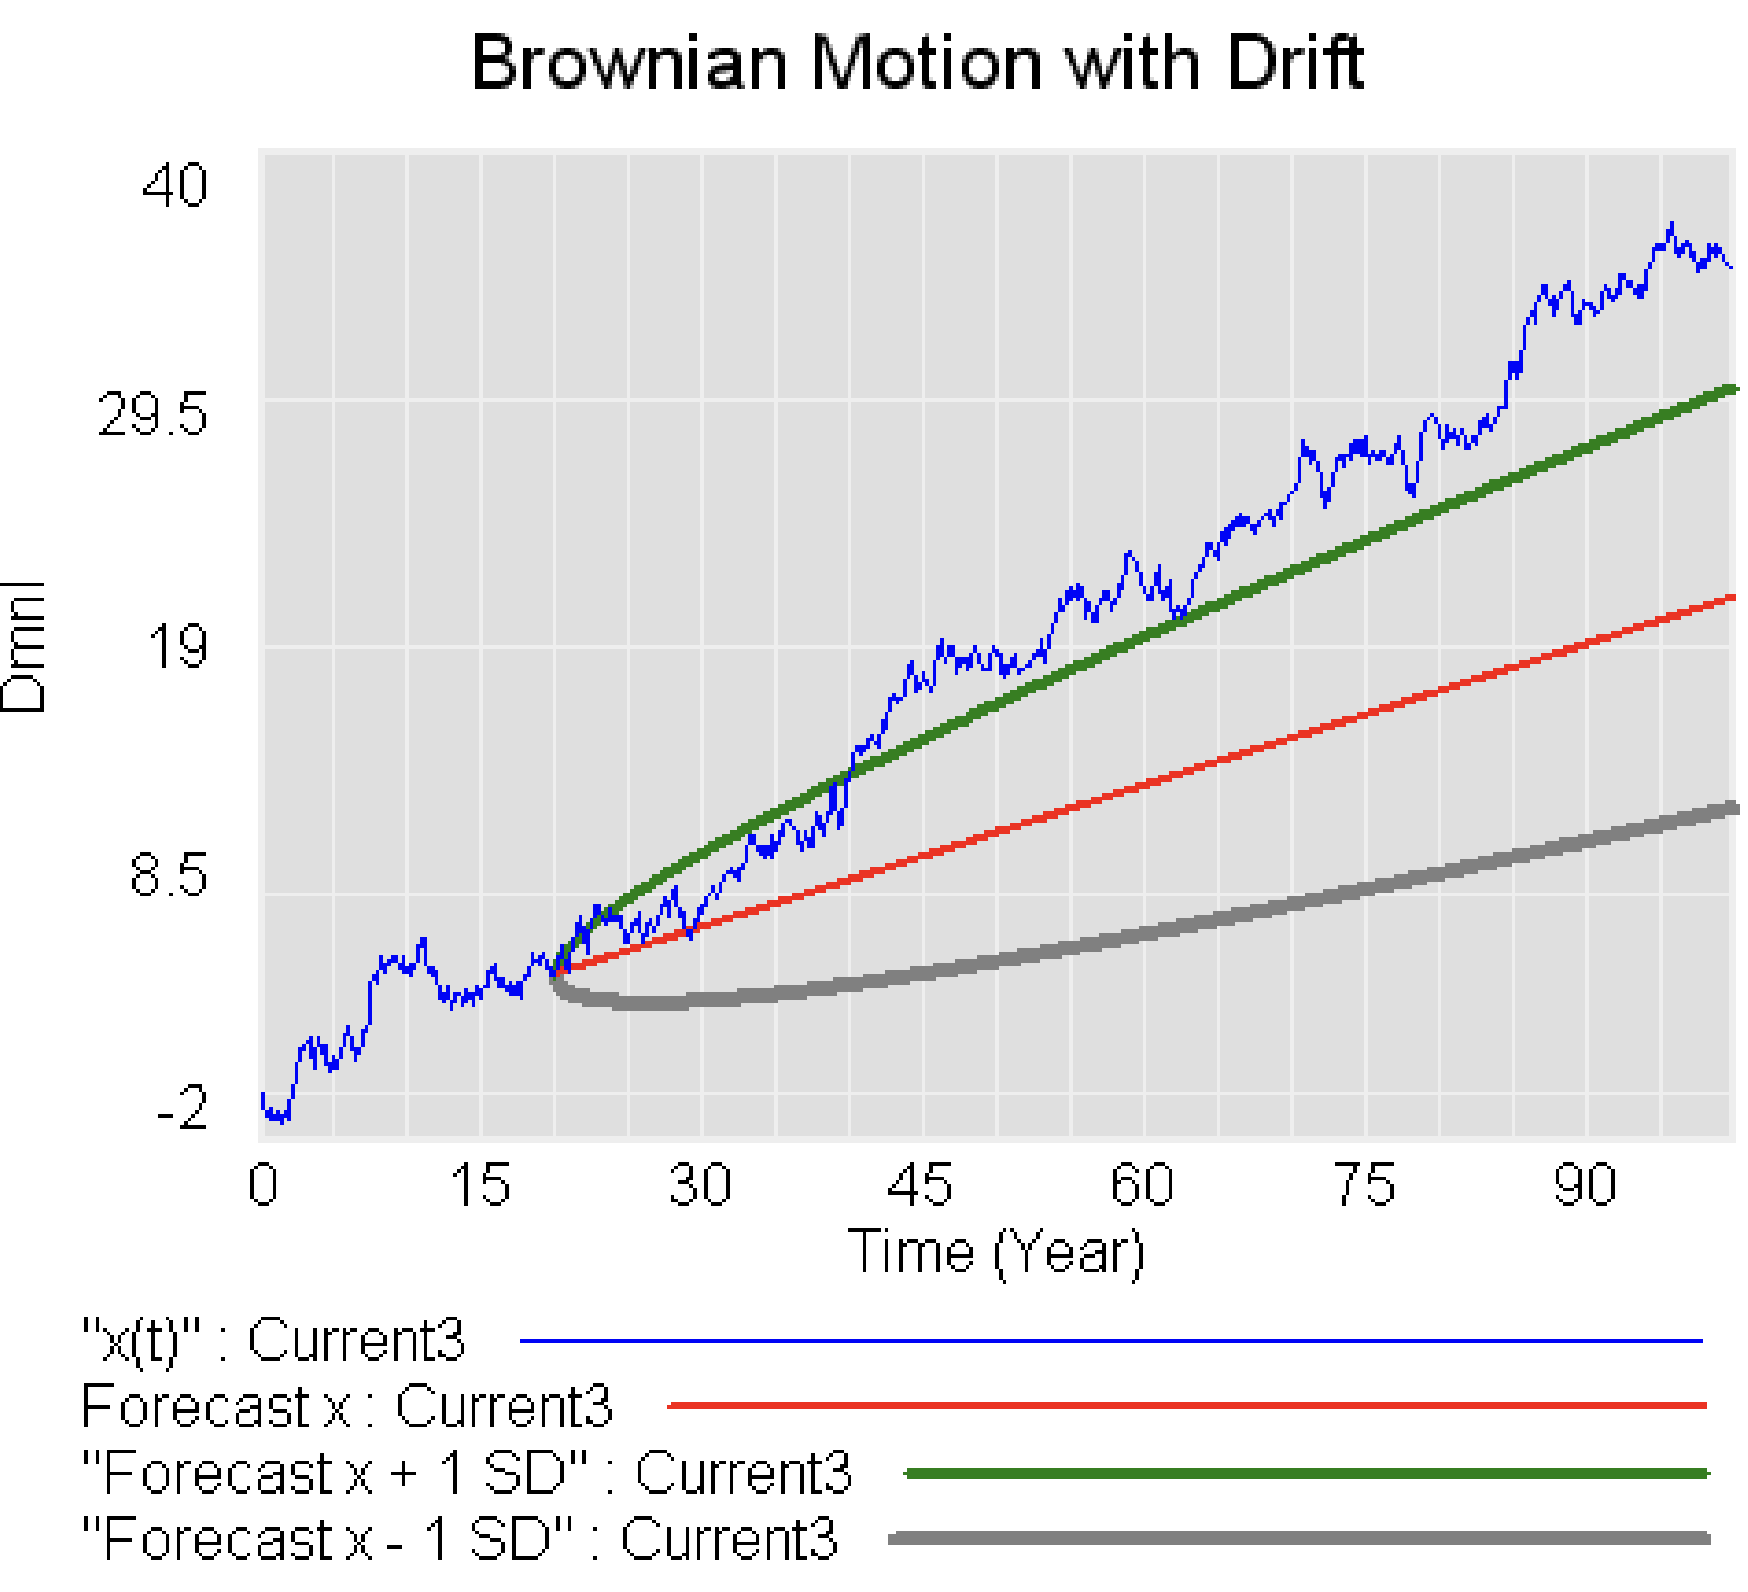
\includegraphics[scale=0.3]{./Brownian6}
	\end{figure}
\end{frame}


%%%%%%%%%%%%%%%%%%%%%%%%%%  SLIDE   %%%%%%%%%%%%%%%%%%%%%%%%%%%%%
\begin{frame}{}

\textbf{Ornstein-Uhlenbeck (OU) process:}
\begin{witemize}
\item Continuous time analog of the AR(1) process
\begin{equation*}
	dz_t = \theta(\bar z - z_t) dt + \sigma dB_t
\end{equation*}

\item Popular model for earnings risk and income fluctuations

\item Auto-correlation of $e^{-\theta} \approx 1-\theta$. Compare to:
\begin{equation*}
	x_{t+1} = \theta \bar x + (1-\theta) x_t + \sigma \epsilon_t
\end{equation*}

\item Stationary distribution is $\mathcal N(\bar z, \frac{\sigma^2}{2\theta} )$

\end{witemize}
\end{frame}


%%%%%%%%%%%%%%%%%%%%%%%%%  SLIDE   %%%%%%%%%%%%%%%%%%%%%%%%%%%%%%
\begin{frame}{}
	\begin{figure}
		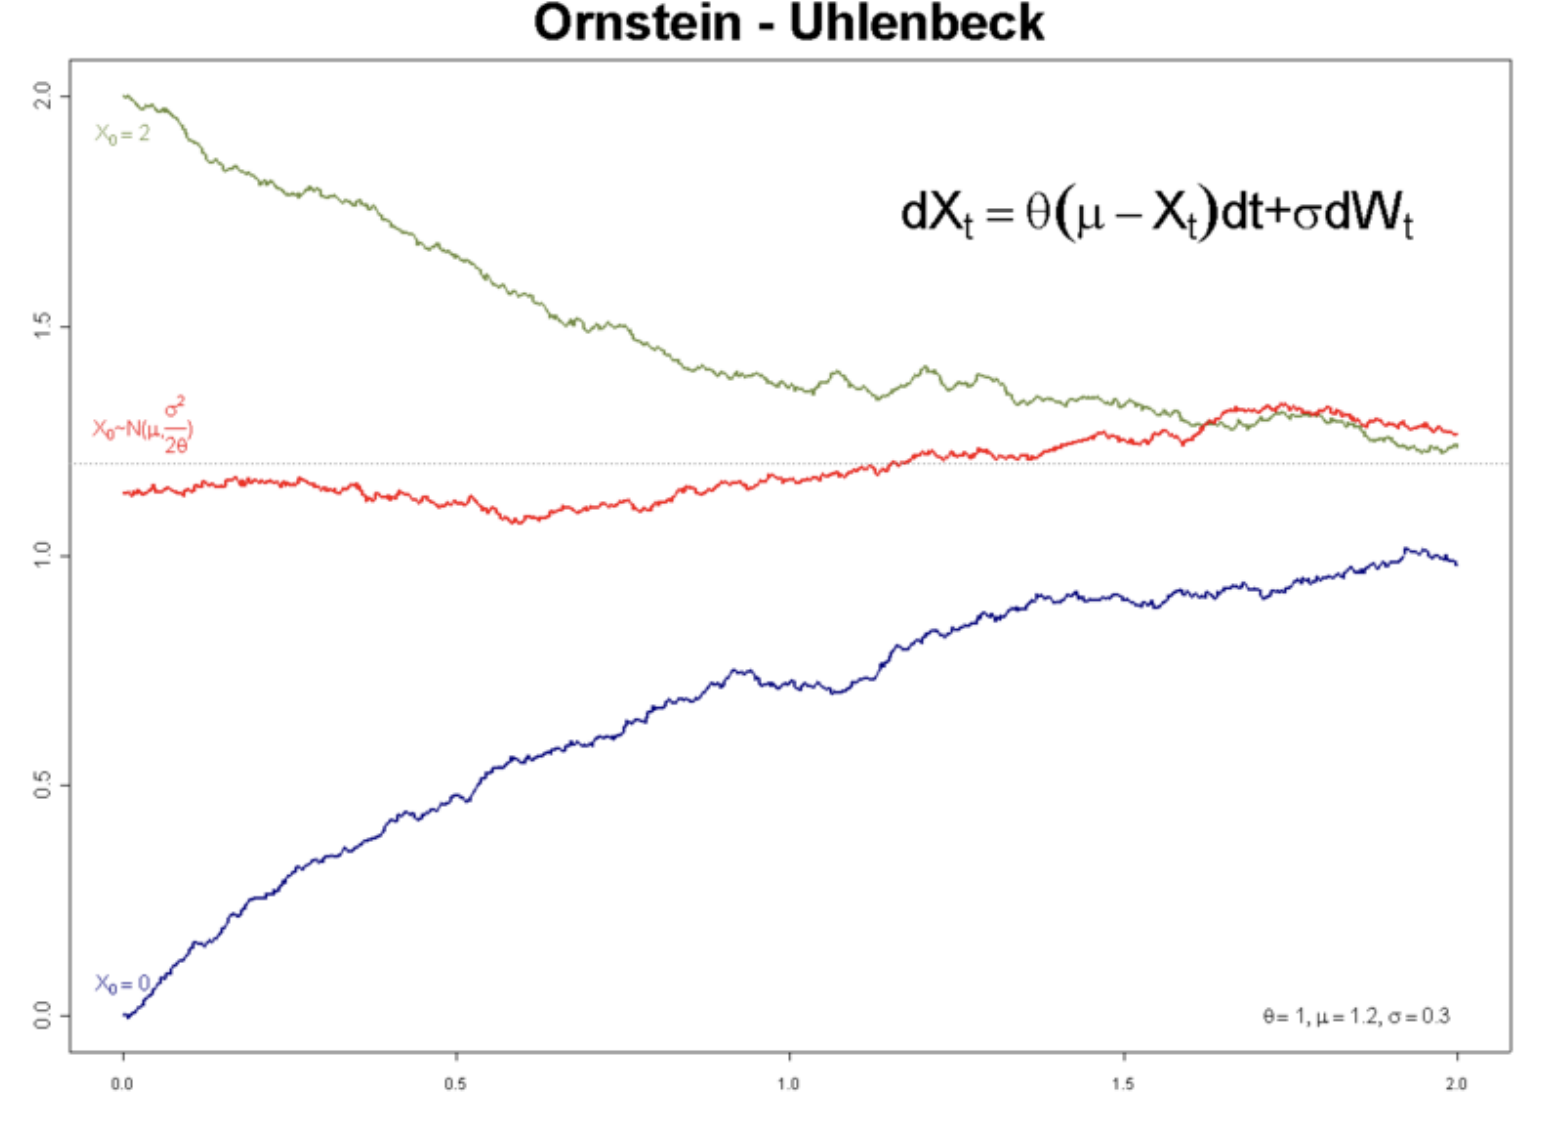
\includegraphics[scale=0.3]{./Brownian7}
	\end{figure}
\end{frame}


%%%%%%%%%%%%%%%%%%%%%%%%%%  SLIDE   %%%%%%%%%%%%%%%%%%%%%%%%%%%%%
\begin{frame}{}

\begin{witemize}
\item Diffusion processes allow us to construct many other processes with desired properties by simply choosing $\mu(t, X)$ and $\sigma(t, X)$

\item Process that stays in interval $[0, 1]$ and mean-reverts around $1/2$:
\begin{equation*}
	dX = \theta( \frac{1}{2} - X)dt + \sigma X(1-X) dB
\end{equation*}

\item Feller square root process (finance: ``Cox-Ingersoll-Ross''):
\begin{equation*}
	dX = \theta(\bar X - X)dt + \sigma \sqrt X dB
\end{equation*}
with stationary distribution $\sim \Gamma\Big( \frac{2 \theta \bar X}{\sigma^2}, \frac{\sigma^2}{2 \theta \bar X} \Big)$

\end{witemize}
\end{frame}




%%%%%%%%%%%%%%%%%%%%%%%%%%  SLIDE   %%%%%%%%%%%%%%%%%%%%%%%%%%%%%%%%
\begin{transitionframe}
	{\color{white} \Large \textbf{Part 2: Optimization with stochastic dynamics} \vspace{2mm}}
\end{transitionframe}


%%%%%%%%%%%%%%%%%%%%%%%%%%  SLIDE   %%%%%%%%%%%%%%%%%%%%%%%%%%%%%%%%
\begin{frame}{1. The generator of a stochastic process}

\textbf{Definition.} The \textbf{generator} of a stochastic process $X$ is defined (for any test function $f$) as
\begin{equation*}
	\mathcal A f = \lim_{\Delta t \to 0} \mathbb E_t \frac{ f(t + \Delta t, X(t + \Delta t)) - f(t, X(t)) }{\Delta t}
\end{equation*}
	
\vspace{5mm}
\begin{witemize}
\item The generator $\mathcal A$ tells us how the stochastic process is \textit{expected} to evolve

\item The generator $\mathcal A$ is a functional operator
\end{witemize}
\end{frame}


%%%%%%%%%%%%%%%%%%%%%%%%%%  SLIDE   %%%%%%%%%%%%%%%%%%%%%%%%%%%%%%%%
\begin{frame}{Generator for diffusion processes}

\begin{witemize}
\item We start with the diffusion process
\begin{equation*}
	dX = \mu(t, X) dt + \sigma (t, X) dB
\end{equation*}

\item On homework, you will show that:
\begin{equation*}
	\mathcal A f = \partial_t f(t, X) + \mu(t, X) \partial_X f(t, X) + \frac{1}{2} \sigma(t, X)^2 \partial_{XX} f(t, X)
\end{equation*}

\item For the general / multi-dimensional version see Oksendal
\end{witemize}
\end{frame}


%%%%%%%%%%%%%%%%%%%%%%%%%%  SLIDE   %%%%%%%%%%%%%%%%%%%%%%%%%%%%%%%%
\begin{frame}{Generator for Poisson processes}
\begin{witemize}
\item Next, we consider the poisson process $\{ Y_t \}$ where $Y_t \in \{ Y^1, Y^2 \}$. This is a two-state Markov chain in continuous time.

\item We assume that the Poisson intensity / arrival rate / hazard rate is $\lambda$

\item The generator is now given by
\begin{equation*}
	\mathcal A f (Y^j) = \lambda \Big[ f( Y^{-j} ) - f (Y^j) \Big]
\end{equation*}

\item Intuition: at rate $\lambda$ you transition, so you lose the value of your current state, $f(Y^j)$, and obtain the value of the new state, $f(Y^{-j})$

\item Again see Oksendal for general version of this and more details
\end{witemize}
\end{frame}




%%%%%%%%%%%%%%%%%%%%%%%%%%  SLIDE   %%%%%%%%%%%%%%%%%%%%%%%%%%%%%%%%
\begin{frame}{2. Stochastic Neoclassical Growth Model}

\textbf{Preferences.} Lifetime utility of representative household 
\begin{equation*}
	\mathbb E_0 \int_0^\infty e^{- \rho t} u(c_t) dt 
\end{equation*}


\vspace{3mm}
\textbf{Technology.} Final consumption good produced using technology 
\begin{equation*}
	y_t = F(k_t, z_t)
	\quad\quad \text{ where } 
	F(0, z) = 0, \text{ and } F_k, F_z > 0, \text{ and } F_{kk} < 0
\end{equation*}
where $z_t$ is exogenous productivity, and capital accumulation technology is 
\begin{equation*}
	dk_t = (i_t - \delta k_t) dt.
\end{equation*}


\vspace{3mm}
\textbf{Resource constraint} for the final good is:  $y_t = c_t + i_t$ 

\vspace{3mm}
\textbf{Endowment.} At time $t = 0$, economy's initial state is $(k_0, z_0)$

\end{frame}


%%%%%%%%%%%%%%%%%%%%%%%%%%  SLIDE   %%%%%%%%%%%%%%%%%%%%%%%%%%%%%%%%
\begin{frame}{}

\textbf{Planning problem.} Taking as given $(k_0, z_0)$, choose an allocation to maximize lifetime utility of representative household subject to technologies and resource constraints:
\begin{equation*}
	V(k_0, z_0) = \max \mathbb E_0 \int_0^\infty e^{- \rho t} u(c_t) dt 
\end{equation*}
subject to 
\begin{align*}
	y_t &= F(k_t, z_t) \\
	y_t &= c_t + i_t \\
	dk_t &= (i_t - \delta k_t) dt \\
	dz_t &\text{ exogenous }
\end{align*}
and taking as given $(k_0, z_0)$

\vspace{2mm}
Combining: \hspace{30mm} $dk_t = [F(k_t, z_t) - c_t - \delta k_t] dt$

\end{frame}



%%%%%%%%%%%%%%%%%%%%%%%%%%  SLIDE   %%%%%%%%%%%%%%%%%%%%%%%%%%%%%%%%
\begin{frame}{3. Productivity as a diffusion process}
\begin{witemize}
\item We start with diffusion process:
\begin{equation*}
	dz_t = - \theta z_t dt + \sigma dB_t,
\end{equation*}
where $\theta$ and $\sigma$ are constants

\item This is a continuous-time, mean-reverting AR(1) process called the Ornstein-Uhlenbeck process

\item State space is now given by
\begin{equation*}
	\Big\{ (k, z) \mid k \in [0, \bar k] \text{ and } z \in [\underline z, \bar z] \Big\}
\end{equation*}
\end{witemize}
\end{frame}


%%%%%%%%%%%%%%%%%%%%%%%%%%  SLIDE   %%%%%%%%%%%%%%%%%%%%%%%%%%%%%%%%
\begin{frame}{}

{\small
\begin{witemize}
\item In discrete time, we would have 
\begin{equation*}
	V(k_t, z_t) = \max_c \Big\{ u(c) \Delta t + \frac{1}{1 + \rho \Delta t} \mathbb{E}_t V(k_{t + \Delta t}, z_{t + \Delta t} ) \Big\}
\end{equation*}

\item Difference from previous lecture: $\mathbb E$ because there is uncertainty
\begin{align*}
	(1 + \rho \Delta t) V(k_t, z_t) &= \max_c \Big\{ (1 + \rho \Delta t) u(c) \Delta t+ \mathbb{E}_t V(k_{t + \Delta t}, z_{t + \Delta t})  \Big\} \\
	\rho \Delta t V(k_t, z_t) &= \max_c \Big\{ u(c) \Delta t+ \mathbb{E}_t V(k_{t + \Delta t}, z_{t + \Delta t} ) - V(k_t, z_t) \Big\} \\
	\rho V(k_t, z_t) &= \max_c \Big\{ u(c) + \mathbb{E}_t \frac{V(k_{t + \Delta t}, z_{t + \Delta t} ) - V(k_t, z_t)}{\Delta t} \Big\}
\end{align*}

\item Take limit $\Delta t \to 0$ and drop time subscripts: 
\begin{equation*}
	\rho V(k, z) = \max_c \Big\{ u(c) + \mathbb{E} \frac{d V(k, z)}{dt} \Big\}
\end{equation*}

\item What remains? Characterizing continuation value $\frac{d}{dt} V(k, z)$ (i.e., characterizing how process $dV$ evolves)

\end{witemize}
}
\end{frame}


%%%%%%%%%%%%%%%%%%%%%%%%%%  SLIDE   %%%%%%%%%%%%%%%%%%%%%%%%%%%%%%%%
\begin{frame}{}
\begin{witemize}
\item The generator $\mathcal A$ is exactly the answer to this question! I.e., 
\begin{align*}
	\mathbb E \frac{d V(k, z)}{d t} &= \mathcal A V(k , z) \\
	&= \Big( F(k, z) - \delta z - c \Big) \partial_k V(k, z) - \theta z \partial_z V(k, z) + \frac{\sigma^2}{2} \partial_{zz} V(k, z)
\end{align*}

\item Therefore, we arrive at the Hamilton-Jacobi-Bellman equation
\begin{align*}
	\rho V(k, z) = \max_c \Big\{ & u(c) + \Big( F(k, z) - \delta z - c \Big) \partial_k V(k, z) \\
	&- \theta z \partial_z V(k, z) + \frac{\sigma^2}{2} \partial_{zz} V(k, z) \Big\}
\end{align*}
with first-order condition 
\begin{equation*}
	u'(c(k, z)) = \partial_k V(k, z)
\end{equation*}
\end{witemize}
\end{frame}



%%%%%%%%%%%%%%%%%%%%%%%%%%  SLIDE   %%%%%%%%%%%%%%%%%%%%%%%%%%%%%%%%
\begin{frame}{4. Productivity as a Poisson process}

{\small
\begin{witemize}
\item Next, consider Poisson process for $\{ z_t \}$ with $z_t \in \{z^L, z^H\}$

\item Generator now given by
\begin{equation*}
	\mathcal A V(k, z^j) = \Big( F(k, z) - \delta z - c \Big) \partial_k V(k, z) + \lambda \Big[ V(k, z^{-j}) - V(k, z^j) \Big]
\end{equation*}

\item Note: derivation of HJB exactly as before \textit{up to} characterizing $\mathbb E [d V]$

\item With Poisson process, HJB becomes
\begin{align*}
	\rho V(k, z^j) = \max_c \Big\{ & u(c) + \Big( F(k, z) - \delta z - c \Big) \partial_k V(k, z) \\
	&+ \lambda \Big[ V(k, z^{-j}) - V(k, z^j) \Big] \Big\}
\end{align*}
with first-order condition 
\begin{equation*}
	u'(c(k, z^j)) = \partial_k V(k, z^j)
\end{equation*}
\end{witemize}
}
\end{frame}



%%%%%%%%%%%%%%%%%%%%%%%%%%  SLIDE   %%%%%%%%%%%%%%%%%%%%%%%%%%%%%%%%
\begin{transitionframe}
	{\color{white} \Huge \textbf{Part 3: Applications} \vspace{2mm}}
\end{transitionframe}


%%%%%%%%%%%%%%%%%%%%%%%%%%  SLIDE   %%%%%%%%%%%%%%%%%%%%%%%%%%%%%%%%
\begin{frame}{1. Consumption-savings with income fluctuations}

{\small
\begin{witemize}
\item Economy is populated by representative household that faces income risk

\item Household accumulates wealth according to
\begin{equation*}
	\dot a_t = r a_t + e^{z_t} - c_t 
\end{equation*}
subject to borrowing constraint $a_t \geq 0$

\item Preferences again: $V_0 = \max \mathbb{E}_0 \int_0^\infty e^{- \rho t} u(c_t) dt$

\item Income follows diffusion process: $d y_t = - \theta y_t dt + \sigma dB_t$

\item Away from borrowing constraint, HJB given by
\begin{equation*}
	\rho V = \max_c \Big\{ u(c) + (r a + e^{z} - c) V_a - \theta z V_z + \frac{\sigma^2}{2} V_{zz} \Big\}
\end{equation*}
with $V_a = \partial_a V(a, z)$ (you'll see this often) 
\end{witemize}
}
\end{frame}


%%%%%%%%%%%%%%%%%%%%%%%%%%  SLIDE   %%%%%%%%%%%%%%%%%%%%%%%%%%%%%%%%
\begin{frame}{2. Firm profit maximization}

{\small
\begin{witemize}
\item Firm maximizes NPV of profit: $V_0 = \max \mathbb{E}_0 \int_0^\infty e^{- r t} \pi_t dt$

\item For now, profit given by: $\pi_t = A_t n_t^\alpha - w_t n_t$ where firm chooses labor $n_t$ \\
Assume $\alpha < 1$, so this is a decreasing-returns production function

\item Firm is small and takes wage $\{ w_t \}$ as given (wages determined in general equilibrium)

\item Productivity follows two-state high-low process, with $A_t \in \{ A^\text{rec}, A^\text{boom} \}$

\item Recursive representation: $A$ is only state variable, $w_t = w(A_t)$
\begin{equation*}
	r V(A^\text{boom}) = \max_n \Big\{ A^\text{boom} n^\alpha - w(A^\text{boom}) n + \lambda \Big[ V(A^\text{rec}) - V(A^\text{boom}) \Big] \Big\}
\end{equation*}
with first-order condition
\begin{equation*}
	n = \bigg(\frac{\alpha A^j}{w(A^j)}\bigg)^\frac{1}{1-\alpha}
\end{equation*}

\end{witemize}
}
\end{frame}


%%%%%%%%%%%%%%%%%%%%%%%%%%  SLIDE   %%%%%%%%%%%%%%%%%%%%%%%%%%%%%%%%
\begin{frame}{3. Capital investment with adjustment cost}

{\small
\begin{witemize}
\item Firm again maximizes NPV of profit: $V_0 = \max \mathbb{E}_0 \int_0^\infty e^{- r t} \pi_t dt$

\item Now: let $\psi(\cdot)$ denote an adjustment cost
\begin{align*}
	\pi_t &= e^{A_t} k_t^\alpha - Q_t \iota_t - \psi(\iota_t, k_t) \\
	d k_t &= (\iota_t - \delta k_t) dt \\
	d A_t &= - \theta A_t dt + \sigma dB_t
\end{align*}

\item Firm is small and takes capital price as given 

\item Recursive representation in terms of $(k, A)$, i.e., $Q_t = Q(k_t, A_t)$
\begin{align*}
	r V(k, A) = \max_\iota \Big\{ &e^{A_t} k_t^\alpha - Q(A) \iota_t - \psi(\iota_t, k_t) + (\iota - \delta k) \partial_k V(k, A) \\
	& - \theta A \partial_A V(k, A) + \frac{\sigma^2}{2} \partial_{AA} V(k, A) \Big\}
\end{align*}
with first-order condition: $Q(k, A) + \partial_\iota \psi(\iota(k, A), k) = \partial_k V(k, A)$
\end{witemize}
}
\end{frame}


%%%%%%%%%%%%%%%%%%%%%%%%%%  SLIDE   %%%%%%%%%%%%%%%%%%%%%%%%%%%%%%%%
\begin{frame}{4. Investing in stocks}

{\small
\begin{witemize}
\item Suppose you optimize lifetime utility $V_0 = \mathbb{E}_0 \int_0^\infty u(c_t) dt$

\item You can trade two assets: riskfree bond (return $r dt$), and risky stock 
\begin{equation*}
	dR = (r + \pi) dt + \sigma dB, \text{ where } \pi \text{ is the equity premium}
\end{equation*}

\item You have wealth $a_t$ and invest a share $\theta_t$ in stocks, thus,
\begin{equation*}
	da_t = \theta_t a_t dR_t + (1-\theta_t) a_t r_t dt + y - c_t
\end{equation*}
or, rearranging, and dropping $t$ subscripts
\begin{equation*}
	da = r a + \theta a \pi dt + y - c + \theta a \sigma dB 
\end{equation*}

\item HJB becomes:
\begin{equation*}
	\rho V(a) = \max_{c, \theta} \Big\{ u(c) + (  r a + \theta a \pi dt + y - c  ) V'(a) + \frac{1}{2} (\sigma \theta a)^2 V''(a) \Big\}
\end{equation*}
with FOCs: (i) $u'(c) = V'(a)$ and (ii) $\theta = -\frac{\pi}{\sigma^2} \frac{ V'(a) }{a V''(a)}$
\end{witemize}
}
\end{frame}


%%%%%%%%%%%%%%%%%%%%%%%%%%  SLIDE   %%%%%%%%%%%%%%%%%%%%%%%%%%%%%%%%
\begin{frame}{5. Real business cycles}
\begin{witemize}
\item Next semester, Yuriy will teach the Real Business Cycle model. This is basically the stochastic neoclassical growth model, estimated to match business cycle moments 

\item Recall that this model is efficient so we can look at the planning problem

\item Preferences are:
\begin{equation*}
	\mathbb E_0 \int_0^\infty e^{- \rho t} u(c_t) dt
\end{equation*}

\item And combining technologies and resource constraints yields:
\begin{equation*}
	dk_t = \Big[ f(k_t, z_t) - \delta k_t - c_t \Big] dt
\end{equation*}

\item Now suppose TFP follows a Feller process: $dz_t = \theta(\bar z - z_t) dt + \sigma \sqrt{z_t} dB_t$
\end{witemize}
\end{frame}


%%%%%%%%%%%%%%%%%%%%%%%%%%  SLIDE   %%%%%%%%%%%%%%%%%%%%%%%%%%%%%%%%
\begin{frame}{}
\begin{witemize}
\item With $dz_t = {\color{blue} \theta(\bar z - z_t) } dt + {\color{red} \sigma \sqrt{z_t} } dB_t$, the HJB is then given by:
\begin{equation*}
	\rho V(k, z) = \max_c \bigg\{ u(c) + \Big[ f(k, z) - \delta k - c \Big] V_k(k, z) + {\color{blue} \theta(\bar z - z) } V_z(k, z) + \frac{1}{2} {\color{red} \sigma^2 z } V_{zz}(k, z) \bigg\}
\end{equation*}

\item We have now seen 3 variants of this model with 3 different assumptions for the process $dz_t$

\item This model is the foundation for business cycle macro 
\end{witemize}
\end{frame}


%%%%%%%%%%%%%%%%%%%%%%%%%%  SLIDE   %%%%%%%%%%%%%%%%%%%%%%%%%%%%%%%%
\begin{frame}{6. AK technology and log utility}
\begin{witemize}
\item Assume that $u(c_t) = \log c_t$ and $f(k_t, z_t) = z_t k_t$

\item Assuming that $dz_t$ follows a stationary diffusion process:
\begin{equation*}
	\rho V(k, z) = \max_c \bigg\{ \log c + \Big[ f(k, z) - \delta k - c \Big] V_k(k, z) + \mu(z) V_z(k, z) + \frac{1}{2} \sigma(z)^2 V_{zz}(k, z) \bigg\}
\end{equation*}

\item Show that the consumption policy function is:
\begin{equation*}
	c(k, z) = \rho k
\end{equation*}

\item As a result, model solution characterized by the two \textit{forward} equations:
\begin{align*}
	dk_t &= (z_t - \rho - \delta) k_t dt \\
	dz_t &= \mu(z_t) dt + \sigma(z_t) dB_t
\end{align*}

\end{witemize}
\end{frame}


%%%%%%%%%%%%%%%%%%%%%%%%%%  SLIDE   %%%%%%%%%%%%%%%%%%%%%%%%%%%%%%%%
\begin{frame}{}
\textbf{Proof:}
\begin{witemize}
\item Guess and verify:
\begin{equation*}
	V(k, z) = v(z) + A \log k
\end{equation*}

\item FOC: 
\begin{equation*}
	u'(c(k, z)) = V_k(k, z) 
	\quad \implies \quad
	\frac{1}{c(k, z)} = A \frac{1}{k}
	\quad \implies \quad
	c(k, z) = \frac{1}{A} k
\end{equation*}

\item Plug back into HJB: 
\begin{equation*}
\rho v(z) + \rho A \log k = \log \frac{1}{A} + \log k + (z - \frac{1}{A} - \delta) k A \frac{1}{k} + \mu(z) v'(z) + \frac{1}{2} \sigma(z)^2 v''(z)
\end{equation*}

\item Collect terms in $\log k$ and confirm $\rho A = 1$. Solve ODE for $v(z)$!

\item Economics: log preferences $\implies$ income and substitution effects of future $z_t$ changes cancel $\implies$ constant savings rate $\rho$
\end{witemize}
\end{frame}



\end{document}
